\documentclass{standalone}

\usepackage{amsmath,amsfonts,amssymb,amsthm,mathtools} 
\usepackage{fontspec}            % пакет для подгрузки шрифтов
\setmainfont{STARWARS}   % задаёт основной шрифт документа

% why do we need \newfontfamily:
% http://tex.stackexchange.com/questions/91507/
\newfontfamily{\cyrillicfonttt}{STARWARS}
\newfontfamily{\cyrillicfont}{STARWARS}
\newfontfamily{\cyrillicfontsf}{STARWARS}
% Иногда тех не видит структуры шрифтов. Эти трое бравых парней спасают ситуацию и доопределяют те куски, которые Тех не увидел.

\usepackage{unicode-math}     % пакет для установки математического шрифта
\setmathfont{Asana Math}      % шрифт для математики

\usepackage{polyglossia}      % Пакет, который позволяет подгружать русские буквы
\setdefaultlanguage{russian}  % Основной язык документа
\setotherlanguage{english}    % Второстепенный язык документа

\usepackage{pgf,tikz,pgfplots}
\usetikzlibrary{arrows,calc}
\usepackage{relsize} 

\usepackage{graphicx} 
\usepackage{rotating}
\usepackage{xcolor}
\usepackage{color}

\definecolor{trapcolor}{HTML}{FFEE36}
\definecolor{trapcolor2}{HTML}{FCDF2B}


\begin{document}

\begin{tikzpicture}[scale=2]
% Admiral Akbar
\node[inner sep=0pt] (russell) at (-0.3,-0.8) {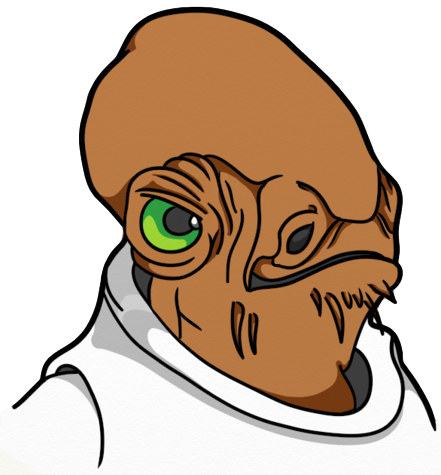
\includegraphics[angle=0,scale=0.2]{new_trap.png}};    

\begin{scope}[rotate=30]   
% Radius of regular polygons
  \newdimen\R
  \R=2cm
  \coordinate (center) at (0,0);
 \draw (0:\R)
     \foreach \x in {60,120,...,360} {  -- (\x:\R) }
              -- cycle (300:\R)
              -- cycle (240:\R)
              -- cycle (180:\R)
              -- cycle (120:\R)
              -- cycle (60:\R)
              -- cycle (0:\R)  [line width=1.9mm,color=black];
\end{scope}       
       
       
\draw[color=black,draw,align=left] (-0.97,0.8) node[scale=1.2,right] { \footnotesize{ $\displaystyle
 \begin{pmatrix}
  1    & x_{1}  & z_{1}  & 0      & 1      \\
  1    & x_{2}  & z_{2}  & 1      & 0      \\
  1    & x_{3}  & z_{3}  & 0      & 1      \\
\vdots & \vdots & \vdots & \vdots & \vdots \\
  1    & x_{n}  & z_{n}  & 0      & 1   
 \end{pmatrix}
$}};        
  
       
% Matrix              
%\draw[color=black,draw,align=left] (-0.97,0.8) node[scale=1.05,right] { \footnotesize{ $\displaystyle
% \begin{pmatrix}
%  1    & x_{21}    & \cdots  & x_{k1}  & 0      & 1      \\
%  1    & x_{22}    & \cdots  & x_{k2}  & 1      & 0      \\
%  1    & x_{23}    & \cdots  & x_{k3}  & 0      & 1      \\
%  1    & x_{24}    & \cdots  & x_{k4}  & 1      & 0      \\
%\vdots & \vdots    & \ddots  & \vdots  & \vdots & \vdots \\
%  1    & x_{2n}    & \cdots  & x_{kn}  &0       & 1   
% \end{pmatrix}
%$}};       

% Caption
\draw[color=black,draw,align=left] (0.55,-0.5) node[right] {\Large IT'S A}; 
\draw[color=black,draw,align=left] (0.5,-0.75) node[right] {\Large TRAP!};     
\end{tikzpicture}



%\begin{tikzpicture}[scale=2]
%% Radius of regular polygons
%  \newdimen\R
%  \R=2cm
%  \coordinate (center) at (0,0);
% \draw (0:\R)
%     \foreach \x in {60,120,...,360} {  -- (\x:\R) }
%              -- cycle (300:\R)
%              -- cycle (240:\R)
%              -- cycle (180:\R)
%              -- cycle (120:\R)
%              -- cycle (60:\R)
%              -- cycle (0:\R)  [line width=3.2pt,color=trapcolor,fill=black,fill opacity=1];
%
%% Admiral Akbar
%\node[inner sep=0pt] (russell) at (0,-0.6) {\includegraphics[angle=0,scale=0.085]{trap2.jpg}};               
%
%           
%% Matrix              
%\draw[color=trapcolor,draw,align=left] (-0.95,0.95) node[right] { \footnotesize{ $\displaystyle
% \begin{pmatrix}
%  1    & x_{21}    & \cdots  & x_{k1}  & 0      & 1      \\
%  1    & x_{22}    & \cdots  & x_{k2}  & 1      & 0      \\
%  1    & x_{23}    & \cdots  & x_{k3}  & 0      & 1      \\
%  1    & x_{24}    & \cdots  & x_{k4}  & 1      & 0      \\
%\vdots & \vdots    & \ddots  & \vdots  & \vdots & \vdots \\
%  1    & x_{2n}    & \cdots  & x_{kn}  & 0      & 1   
% \end{pmatrix}
%$}};       
%
%% Caption
%\draw[color=trapcolor,draw,align=left] (-1,-1.5) node[right] {IT'S A TRAP!};   
%
%\end{tikzpicture}


\end{document}